\chapter{Techniques for Making Attachments to Real World Objects}
Current 3D printing process has the problem of being detached from real world objects, primarily because existing use of 3D printing technology primarily focuses on creating new objects from scratch. This oversimplified assumption precludes the possibility that existing objects can also be extended, repaired or more generally modified to fulfill additional purposes. Being able to augment these existing objects rather than remaking them presents a more sustainable option for fabrication and, further, avoids unnecessarily replacing objects that might be of personal value to the users.

To explore the possibility of augmenting real world objects, one fundamental `prerequisite' is the ability to attach new 3D printed parts or components to existing objects. Fabricating parts to augment existing objects would require amongst other things an understanding of what attachment techniques can be used to join one object to another. There are a myriad of ways to fasten or attach two objects together from anchor bolts to zippers (see for example: \cite{barrett1990fastener, wiki:Fastener}). In our everyday life, this is often achieved using adhesives or fasteners. Adhesives are easily available and easy to use, however to achieve certain reliability one needs to know what kind of adhesive to choose based on the surfaces it is applied to, and further know and apply proper procedures (such as waiting an appropriate amount of time for full curing),. Fasteners are mostly mechanical and often require special structures (e.g., bolt holes, flat surface to be clamped on) within an object to achieve robust fastening. Thus both options are can provide general solutions, but may be difficult to adapt to individual objects' specific geometric and material properties. In particular, objects' geometry might affect the viability (is a certain area attachable?), durability (is the attachment durable?), and usability/semantics (how would an attachment support or hinder the usage of the object?). Overall, how can we leverage the power of 3D printing to address these issues of attaching augmentations to existing objects?

In this chapter, I explore three specific attachment techniques enabled by a unified computational framework: {\em (i)} Print-Over prints attachments directly onto the surface of an object, such as printing a magnet holder to a Teddy bear (Figure~\ref{fig:encore_overview}b); {\em (ii)} Print-to-Affix fabricates parts which are separately attached using straps or adhesive, such as adding a structure to make a glue gun stand (Figure~\ref{fig:encore_overview}c); {\em (iii)} Print-Through prints an attachment through and around a hole of an existing object to interlock with it, such as printing a label into a the handle of a pair of scissors (Figure ~\ref{fig:encore_overview}d).

\begin{figure*}[h]
  \centering
  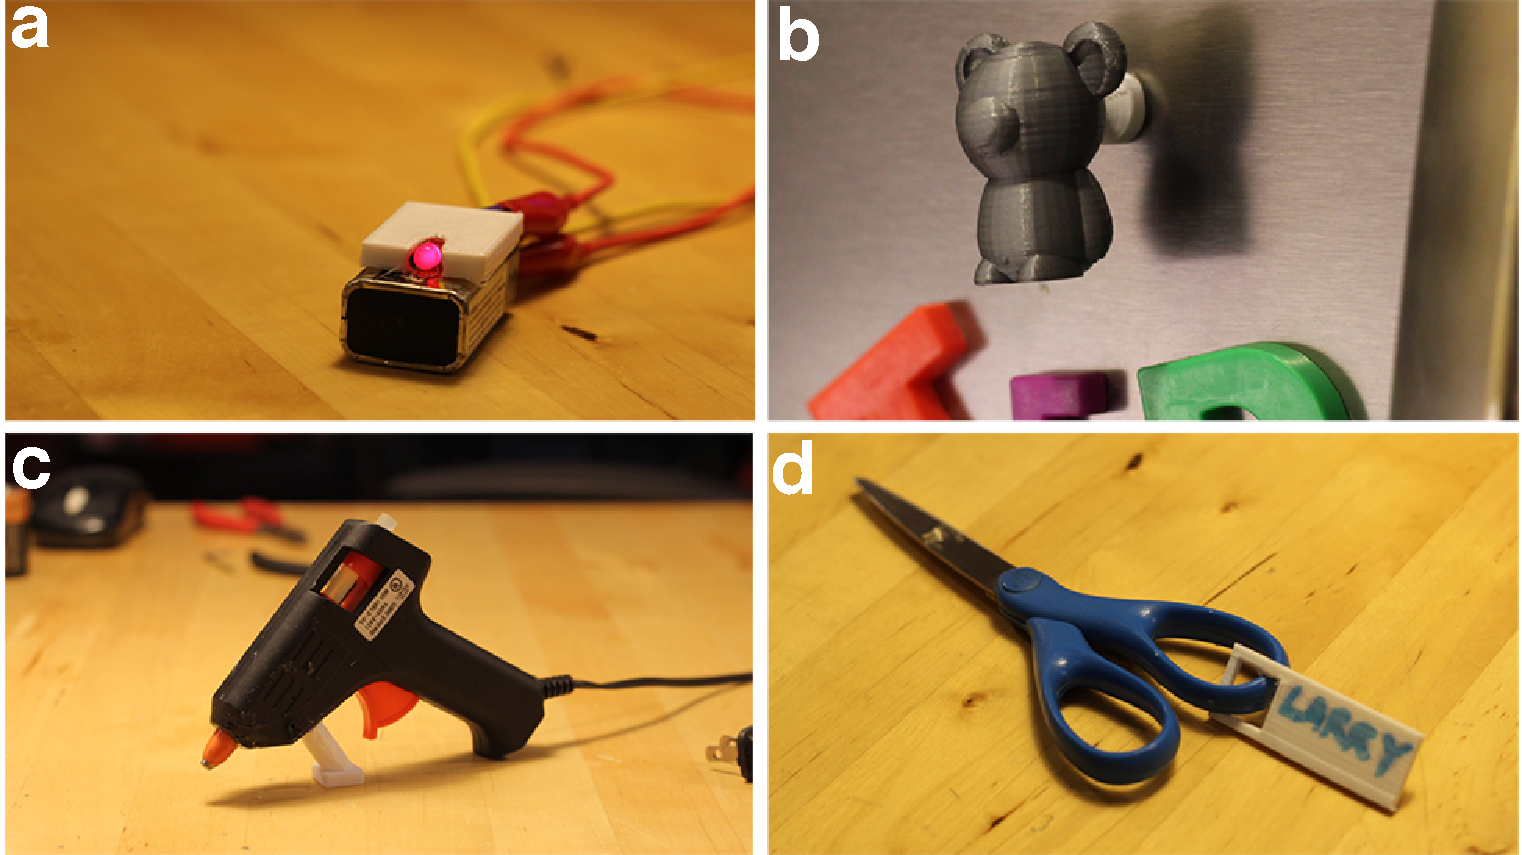
\includegraphics[width=0.8\textwidth]{figures/encore_overview.pdf}
  \caption{Examples of how existing objects can be augmented using our techniques: a) turning a battery into a LED torch; b) making a magnet from a Teddy bear; c) adding a stand to a glue gun and d) attaching a name tag to a pair of scissors. }~\label{fig:encore_overview}
\end{figure*}


These attachment techniques were integrated into Encore--a tool that can import a 3D model of an existing object, perform geometric analyses for the attachment techniques, and allow user exploration through visualization and direct manipulation. Our analysis metrics are designed to provide up-front information about viability, durability and usability of the attachments, where the user can explore tradeoffs among these metrics. Finally, Encore will generate a production-ready model of the parts to be printed, including information necessary for the custom printing process. Figure~\ref{fig:encore_overview} shows an overview of the underlying framework.

\begin{figure*}[h]
  \centering
  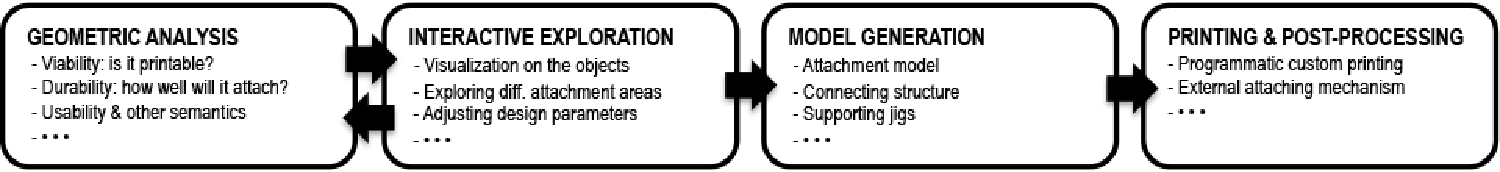
\includegraphics[width=\textwidth]{figures/encore_workflow.pdf}
  \caption{A computational pipeline for designing and fabricating attachments to augment everyday objects. }~\label{fig:encore_workflow}
\end{figure*}

In the remainder of the chapter, I first review existing attachment solutions and how they might afford end-user customization. Then I present the attachment techniques, describe several exemplar analysis metrics for evaluating the goodness of attachment, and present Encore's visualization and direct manipulation interface. Finally I report an evaluation of printing cost and strength.


\section{Existing Attachment Solutions}
Attachment--fastening or otherwise binding two objects together--is a task that commonly arises in everyday life, and one that is not entirely straightforward. Material properties, strength, usability, and aesthetics all need to be considered when attaching objects together. To address this, websites like ThisToThat \footnote{\url{http://www.thistothat.com/}} let a person enter two materials and suggests the best option for gluing them together. Other approaches leverage objects' mechanical properties, such as the widely used joineries and fasteners commonly used in various manufacture industries (e.g., \cite{barrett1990fastener}). Attachment can also be made complex by the specific constraints of the objects being connected. For example, the free universal construction kit\footnote{\url{http://fffff.at/free-universal-construction-kit}} offers adaptors between 10 otherwise incompatible children's construction kits from Lego™ to Tinker toys.

In this work, we are primarily interested in attaching 3D printed components to existing objects. We assume that the existing object is not designed with attachment in mind, and is not to be directly modified (e.g., by drilling holes in order to use a bolt). Specifically, given an existing object and a new part we would like to fabricate and attach, we can either create a binding force between the new part and the old (such as using adhesives, or printing directly over a material that the filament will easily adhere to it) or in some cases we can loosely interlock the new part and the old (such as a buckling a strap through a handle or adding a charm to a charm bracelet or a key to a ring).

Choosing among these forms of attachment is a matter of understanding the task to be accomplished and the constraints that come with it. For example, if we wish to add a doggie bag holder to a dog leash, we may want it to be removable, but not moveable once attached (so it doesn't flap around too much). It must be sturdy enough to survive many walks, dropped leashes, and so on, but does not need to carry much weight (just a roll of plastic bags). It may need to attach just below the handle of a cloth leash, or perhaps we are designing one that can attach to the plastic handle of a retractable leash. As another example, if we wish to add a handle to an espresso cup, it should withstand sheer forces based on the typical weight of a cup. These examples clearly demonstrate the wide range of issues that must be considered, and the interaction of properties of the existing object, task, and object to be attached.

To summarize, to determine the goodness of an attachment technique, viability, durability and usability are all important, although their relative importance may vary. Keeping these issues in mind, our focus in this project is on attachments to, around, or through an existing object without modification by leveraging the fabrication process and customizability of 3D printing. Below I showcase three exemplary attachment techniques.

\section{Techniques For 3D Printed Attachment}
Our techniques allow attachments to be printed directly onto an existing object (print-over), or separately and then adhered or strapped to it (print-to-affix), or through and around the object's holes (print-through). Here we assume that the models of the existing and the new objects have been acquired using 3D scanning, or created from scratch, and focus on methods for attaching the two together.

\subsection{Technique \#1: Print-Over}
The first technique, print-over, is able to print an attachment directly onto the existing object. Once the attachment location is specified, the existing object is oriented and scaffolded with support structures so that it will not move while the attachment is printed on it. It is also important to ensure that the existing object will not impede the motion of the print head while the attachment is being printed.

Figure~\ref{fig:encore_overview}b shows a magnet holder directly printed over a Teddy bear toy (in this case also 3D printed) to make it a fridge magnet. As shown in Figure~\ref{fig:encore_techniques}a, this was done by scaffolding the Teddy bear to the print bed so that the attachment area is facing upward and is accessible by the extruder, which then prints the magnet holder.

\begin{figure*}[h]
  \centering
  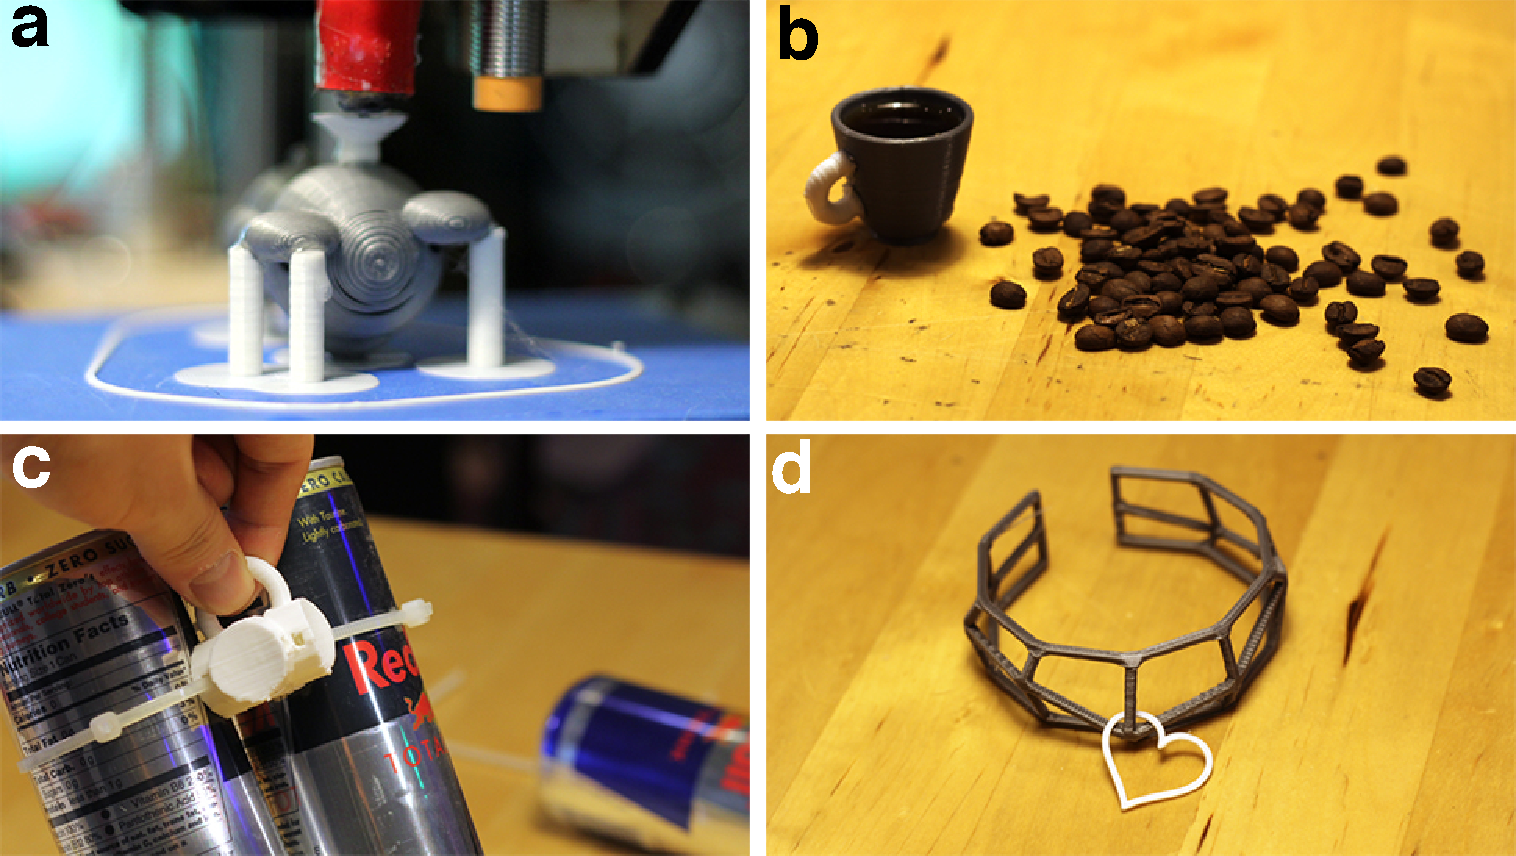
\includegraphics[width=0.8\textwidth]{figures/encore_techniques.pdf}
  \caption{a) The magnet holder printed directly on a teddy bear that was scaffolded on support structures; b) a handle added to an espresso cup; c) strapping to make a reusable “4 pack” handle; and d) a bracelet printed through a heartshaped charm. }~\label{fig:encore_techniques}
\end{figure*}

Print-over works well when the attachment and the existing object are made of the same material, or materials that share similar thermodynamic properties. As detailed later, our evaluation shows that print-over is strong enough to sustain stress as if they had been printed in one piece. When objects are made of less compatible materials, we employ a work-around to perform print-over. Figure~\ref{fig:encore_overview}a shows an LED casing printed directly over a 9V battery to make a simple torch. This was done by adding a thin layer of glue on the battery prior to printing the casing. The glue simply creates a plastic-like layer that allows the printer's material (PLA) to stick to the battery while being printed.

\subsection{Technique \#2: Print-to-Affix}
The second technique, print-to-affix, makes use of the concept of a connector that confomrs to the surface geometry of the existing object and is snug-fit to the new object. This connecter can be printed separately and then attached using external mechanisms (e.g., glue, or straps). This leverages the customizability of 3D printing to bridge objects and attachments that by default are likely to have unmatching surfacing. Figure~\ref{fig:encore_techniques}c shows connectors used for the handle attachment to hold it tight with cans. Print-to-affix is a very general technique and can encompass for example the use of adhesive, straps, or even a custom printed part that snaps into place in some way. It also has the advantage of not preferring the existing object to be flat, as there is no concern about the print head colliding with the existing object.

Figure 1c shows a structure added to a glue gun to make it stand. This geometry was made to precisely match the attaching part on the glue gun, then 3D printed, and attached using adhesive. However, one disadvantage of using adhesive (or the aforementioned print-over) is the difficulty in detaching the attachment for redesign or reuse. Affixing with straps solves this problem. For example, using straps for the `4 pack' holder in Figure~\ref{fig:encore_techniques}c makes this handle reusable without either breaking it or the cans it holds.

Print-to-affix includes a wide variety of options. Details such as whether adhesives or straps are used significantly change the properties of the resulting attachment. For example, in one experiment, a 150mm zip tie could sustain up to a 4kg pulling force before the test object slipped, while the particular adhesive we applied tended to break at a less than 1kg force. On the other hand, using adhesives is less noticeable from an aesthetic standpoint.

\subsection{Technique \#3: Print-through}
The third technique, print through, leverages the structural holes in some existing objects (e.g., keys and rings) to print the attachment through and around it. To accomplish this, the attachment is partially printed, the existing object is placed, and then printing continues until the two objects are interlocked and the print is complete. This requires determining whether there is a viable point at which to stop the print, and whether once the existing object is placed it will interfere with the print head.

Figure~\ref{fig:encore_overview}d shows a name tag printed through the handle of a pair of scissors. As shown in Figure~\ref{fig:encore_printthru}, this was done by programmatically pausing the printer at a point where the scissors can be placed down and out of the way of the print head. Print-through has aesthetic qualities that distinguish it from print-to-affix and print-over: it typically creates a loose but permanent connection between two objects. Figure~\ref{fig:encore_techniques}d is another such example whereby a bracelet was printed through a charm.

\begin{figure*}[h]
  \centering
  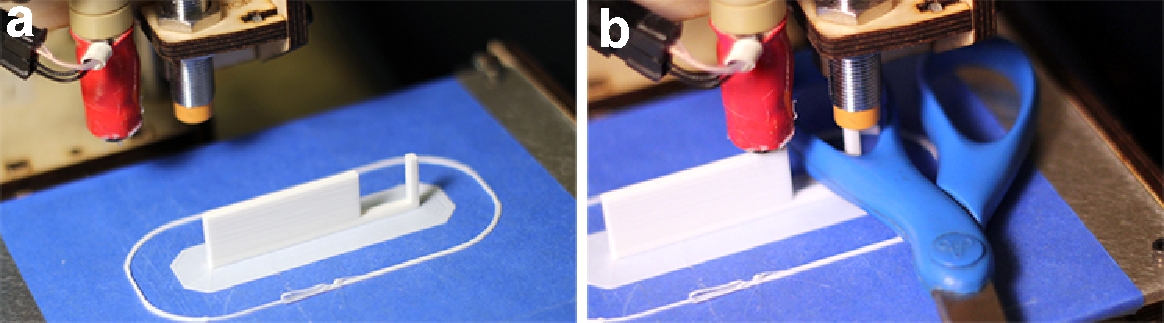
\includegraphics[width=0.8\textwidth]{figures/encore-printthru.pdf}
  \caption{Example of a print-through process: the printer pauses at a point where the scissors can be dropped to interlock with the name tag, after which the print job resumes. }~\label{fig:encore_printthru}
\end{figure*}

As highlighted in the techniques just presented, a range of tradeoffs must be considered when creating 3D printed attachments to existing objects. To address this, we present a series of analysis, based on the geometric properties calculated over the triangular meshes representing the existing object and the attachment. These analyses represent a sample of metrics that pertain to viability, durability, and usability. However, it is our intent and expectation that this set would be expanded over time and as new attachment techniques are explored.

\begin{itemize}
	\item \textit{Viability} indicates whether it is possible for a new part to be fabricated and attached at a given location on an existing object. For example, collision with the extruder during a direct print over process would violate viability;
	\item \textit{Durability} examines how the geometric properties of the contact area between the attachment and the object could potentially strengthen or weaken the bond between them;
	\item \textit{Usability and other semantics} considers various issues related to the actual usage of the attachment, such as the forces we expect to be applied to it, its balance, and some technique-specific issues (such as the length of strap required for fastening an attachment).
\end{itemize}

The next section will describe the details of these analyses, which serve as the computational backend of Encore---an interactive tool that informs people how attachments can be added to existing objects and how well they will perform in terms of viability, durability, usability and other semantics.


\section{Geometric Analysis: Viability}
Viability can encompass issues such as appropriateness for a specific printer with regard to issues such as support or size, as well as feasibility of printing without collision when an existing object is present during printing. Our work focuses on this last issue, which arises during print-over and print-through.
More specifically, when printing involves two objects, it is only viable if {\em (i)} the attachment can be printed without the extruder's tool paths colliding with the existing object (extruder-object collision); {\em (ii)} the attachment and the existing objects also do not intersect and collide with each other for a given spatial configuration (object-object collision). As shown in this section, both types of collisions are affected by the position and orientation of the existing object and the attachment. Thus, we must determine a position and orientation of both objects where the attachment can be printed collision-free.

\subsection{Understanding Viability: Collision Detection}
The first step of viability analysis is to detect collisions that will prevent the attachment from being printed.

\subsubsection{Detecting Extruder-Object Collision}
Extruder-object collision occurs when the placement of the existing object impedes the printer's extruder movement while the attachment is being printed. This type of collision problem is very common in subtractive manufacturing and is often solved by careful tool path planning \cite{chih1998new, lin1996efficient}, such as controlling the path of the cutting bit on a CNC router to avoid running into parts that are not to be removed. WirePrint has shown that collision can be avoided in non-layered additive manufacturing by modeling and considering the geometry of the extruder and the object \cite{mueller2014wireprint}. In print-over, given an attachment $\Lambda$ to an existing object $\Omega$, we scan all $\Omega$'s' vertices above the attaching point to detect whether they are within the range of the extruder's movement, which can be obtained by computing the bounding radii of both the extruder and $\Lambda$.

\subsubsection{Detecting Object-Object Collision}
We consider and address two forms of object-object collision between an attachment and an existing object.

\textbf{Direct Collision}. In an interface for attachment placement, the mapping of the 3D scene onto a 2D screen could cause user errors in the placement of $\Lambda$ with respect to $\Omega$. A user might perceive $\Lambda$ as interlocking with $\Omega$, and yet the two in fact slightly intersect with each other, such that $\Lambda$ is unable to be fabricated (Figure~\ref{fig:encore_feedback}).

\begin{figure*}[h]
  \centering
  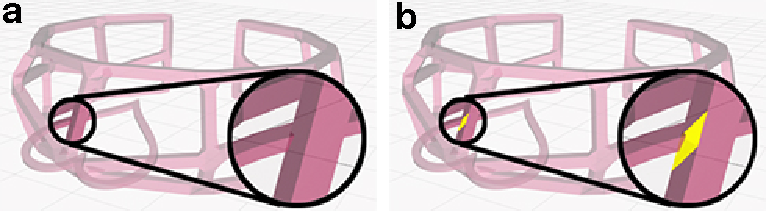
\includegraphics[width=0.75\textwidth]{figures/encore_feedback.pdf}
  \caption{Print-through provides visual feedback (highlighting intersecting faces) to inform users of object-object collision that might not look obvious from certain viewing angle. }~\label{fig:encore_feedback}
\end{figure*}

Such direct object-object collision is commonly dealt with using approximate models (e.g., checking axis-aligned bounding boxes for collision \cite{bergen1997efficient}). Such models could be problematic for attachments: for example, in print-through, $\Lambda$ and $\Omega$ can be interlocking and collision free even though their bounding boxes do intersect with one another.

To address this, we compute whether two objects truly intersect by analyzing their meshes. To narrow down the detection scope, we compute both $\Lambda$ and $\Omega$'s bounding spheres and locate a set of ‘mutually bounded' faces from $\Omega$, denoted as $F^\Omega$. Essentially, $\Lambda$ and $\Omega$ are intersection free if and only if none of $F^\Omega$'s faces intersect with $\Lambda$'s. By walking through a pre-computed octree of $\Lambda$ \cite{meagher1980octree}, we can determine if a given face of $F^\Omega$ intersects with $\Lambda$. Further, as detailed later, we can also visualize the intersecting areas to inform the users how to reposition the attachment to an occlusion-free location (Figure~\ref{fig:encore_feedback}).

\textbf{Indirect Collision}. When objects need to be placed around or through another object (e.g., a partial print), indirect collisions can occur. For example, viability is violated in print-through if one object cannot be moved to its intended interlocked position without ‘passing through' (i.e., intersecting) the body of the other object.

Figure~\ref{fig:encore_interlockable} shows an artificial print-through example to explain this problem. In Figure~\ref{fig:encore_interlockable}a, the existing object (the torus) cannot be inserted into the larger structure (building layer by layer in the direction of the arrow) no matter when the printer is paused. Note that as illustrated in Figure~\ref{fig:encore_interlockable}b, indirect collision is orientation dependent – there might exist an orientation that does provide a viable print for some pause point, different than the one specified by the user for analysis.

\begin{figure*}[h]
  \centering
  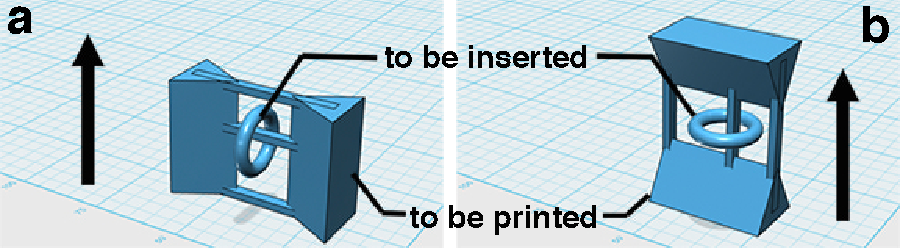
\includegraphics[width=0.75\textwidth]{figures/encore_interlockable.pdf}
  \caption{Interlocking objects are not always viable for printing: a) the torus cannot be inserted while the structure is being printed due to collision; b) a different orientation makes the print viable. (arrows indicate printing directions).}~\label{fig:encore_interlockable}
\end{figure*}

Inspired by Zhou et al.'s use of physics to unfold an object so as to test whether it can be folded \cite{zhou2014boxelization}, we make use of a reverse physics simulation. Specifically, we test whether there is a viable path for moving the existing object to its desired location (e.g., the scissors in Figure~\ref{fig:encore_printthru}) partway through the print of the new object. We test such viability by reversing the insertion process. It starts with an object already inserted into the partial print, which is obtained by slicing the whole print so that its top layer is just above the inserted object. Then gravity is reversed. If the object `escapes' under the reversed gravity, there exists a path for it to be inserted back from above and end up at the same placement where the test started.

In cases where this test fails (i.e., the object is trapped in the partial print), we can also perform a binary search to find a viable printing orientation, which we discuss next.

\subsection{Attaining Viability: Resolving Collision}
Once collision is detected, our analysis also searches for a solution by exploring alternate positions and orientations.

\subsubsection{Resolving Extruder-Object Collision}
Extruder-object collision is only an issue when printing an attachment $\Lambda$ after an existing object $\Omega$ has been placed. Given a candidate surface area $S$ of $\Omega$ on which $\Lambda$ is to be printed, the first step is to rotate $\Omega$ so that $S$ is relatively level and facing upward for extruder to print $\Lambda$ on (e.g., the Teddy bear in Figure~\ref{fig:encore_techniques}a). Generally $S$ is not a perfectly flat surface to print on, so our next step raises $\Lambda$'s first printing layer $P_0$ to be above the entire $S$. However, after these two operations, printing $\Lambda$ might still run into object-extruder collision if parts of $\Omega$ are also above $P_0$. To address this issue, we first print a connector on $P_0$--a cylindrical structure that is small enough to be printed without collision. These connectors serve to continue raising the starting layer until $\Lambda$ can be printed collision-free. One potential issue of this approach is the strength of these connectors in supporting $\Lambda$, which we also discuss later in the durability analysis section.
Even with these solutions, some surface areas, such as those with a high convexity, might still be unprintable. As detailed later, our exploration phase (Figure~\ref{fig:encore_workflow}) visualizes this information to guide the user in selecting alternate viable attachment areas.

\subsubsection{Resolving Object-Object Collision}
For object-object collision, a search for the position and orientation of $\Lambda$ can determine whether there is a viable solution (in which the ‘reversed gravity' test succeeds). A simplified example of this situation is shown in Figure~\ref{fig:encore_interlockable}, where rotating $\Lambda$ by 90 degrees resolves the issue.

Formally stated, the goal is to find a pair of rotations $(\alpha, \gamma)$ such that there exists a viable pause point for $R_x(\alpha)R_y(\gamma)\Omega$. ($R_x$ and $R_y$ are rotation matrices around $x$ and $y$ axis, respectively; rotating around $z$ axis would not change the viability). The solution space is naturally continuous: given an pair of viable $(\hat{\alpha}, \hat{\gamma})$, there must also exist intervals $\alpha_l < \hat{\alpha} < \alpha_u$ and $\gamma_l < \hat{\gamma} < \gamma_u$ such that any printing direction in $\{(\alpha, \gamma) | \alpha_l < \alpha < \alpha_u, \gamma_l < \gamma < \gamma_u \}$ is also viable. Our search process is akin to a binary search of such intervals.

To sum up, the viability analyses described above detect collision issues that arise while fabricating the attachment – either with the extruder or the existing objects. To prevent collision, we can orient the object or raise the starting layer. We also show that a collision-free printing orientation belongs to a continuous solution space and can be found via a binary search.

\section{Geometric Analysis: Durability}
Once a new part is viable for fabrication, the next question is its durability: how well it will attach to the existing object. One simple way to measure durability is to consider the contact area $S$ between the existing object and the attachment; however our framework is extensible to other models and methods such as the cross-sectional analysis \cite{umetani2013cross} and Finite Element Method \cite{szabo1991finite}. Specifically, given a candidate contact area $S$, we consider the following metrics.

\subsubsection{Size}
Size can be approximated by summing up the area of each triangle in or intersecting with $S$. To generalize to multiple attachment sizes, we normalize the measurement by the volume V of the attachment. This metric serves as a simple way to capture an approximation of the structural strength of the connection point with respect to the attachment.

\subsubsection{Flatness}
Flatness can be computed by summing up the vertex-wise distance between $S$ on the existing object and the printing layer at the bottom of the attachment. The flatness score is highest when $S$ is perfectly flat (coplanar with P); and lower as $S$ becomes more irregular, meaning the triangles in $S$ have highly variable heights and orientations, or $S$ has an overall higher curvature.

\subsubsection{Direction and Area of Force}
The relationship between force and strength is affected by the type of attachment being used. For example, techniques such as print-over and using adhesives use interfacial bonds, with adherence to both the existing object and the attachment. In contrast, attachment techniques such as strapping create a force that holds the attachment onto the existing object, which can be measured as follows.

Consider an attachment surface $S$ on the existing object for a strap, we compute $S$'s convex hull $ConvHull(S)$ using a Graham scan \cite{graham1972efficient}. For each point p in $S$, we compute its shortest distance to $ConvHull(S)$: if the distance is smaller than a threshold we consider p to be making contact with a strap around $S$. The object is more strappable at $S$ if most of $S$'s points make contact with the strap. A further consideration is contact point distribution: more evenly distributed contacts suggest a more balanced strapping force.

To sum up, durability examines how the geometric properties of the contact area between the attachment and the object could potentially strengthen or weaken the bond between them. Our analysis shows how contact area and size can be used to compute durability (most usefully for adhesion-based attachments) and explores the metric of strappability, which captures the contact area and force associated with a strap.

\section{Geometric Analysis: Usability \& Semantics}
Even for a new part that is viable and durable, there are often further considerations related to the actual usage of the attachment. We provide two exemplar analysis of usability and semantics: {\em (i)} for handle-like attachments, we consider whether its attachment point creates a balance of the entire object when being gripped or held; and to illustrate a metric which is highly specific to one attachment technique {\em (ii)} an aesthetic strap length metric.

It is only natural that the analysis of usability and semantics would be highly specific to the type of attachment being used. For example, Pr\'evost et al. discuss geometric modifications that can achieve balance such that an object will stand without falling \cite{prevost2013make}. Thus, the metrics we present are by no means exhaustive for the usability and semantic aspects of attachments; rather they suggest exemplar analysis that goes beyond the stage of fabrication and considers the effects and tradeoffs for an attachment in use.

\subsubsection{Balance When Holding an Object By the Attachment}
Balance when holding an object by a given attachment can be measured by moment, which indicates the tendency of the held object to rotate under its own weight. For example, as shown in the ‘4 pack' holder in Figure~\ref{fig:encore_techniques}b, if the handle is rotated 90 degrees, it would be more difficult to hold the cans. When there are multiple contact points selected (such as the handle on an espresso cup), we simply sum up the moments of these points before normalization.

\subsubsection{Technique Dependent Usability Analysis: Strap Length}
Some attachment techniques may make use of very specific usability analysis. For example, the length of the strap is directly related to fastener cost and object appearance. In particular, we consider an analysis of strap length for a candidate attachment configuration normalized to a baseline (e.g., the bounding sphere of the existing object). The strap length can be computed from the aforementioned convex hull of the strapping area.

\section{A Pipeline For Printed Attachments}
We have presented a series of geometric analysis that can be used to quantify the goodness of various potential attachment options from the perspective of viability, durability, and usability. As shown in Figure~\ref{fig:encore_workflow}, analysis results can be integrated into a pipeline for supporting iteration, interactive exploration, model generation, printing and post-processing. We illustrate these phases of the pipeline with our implemented tool, Encore.

\subsection{Interactive Exploration}
The interactive exploration phase creates a feedback loop wherein a user can explore different design parameters. Encore provides visualization and direct manipulation techniques to facilitate this process.

\begin{figure*}[h]
  \centering
  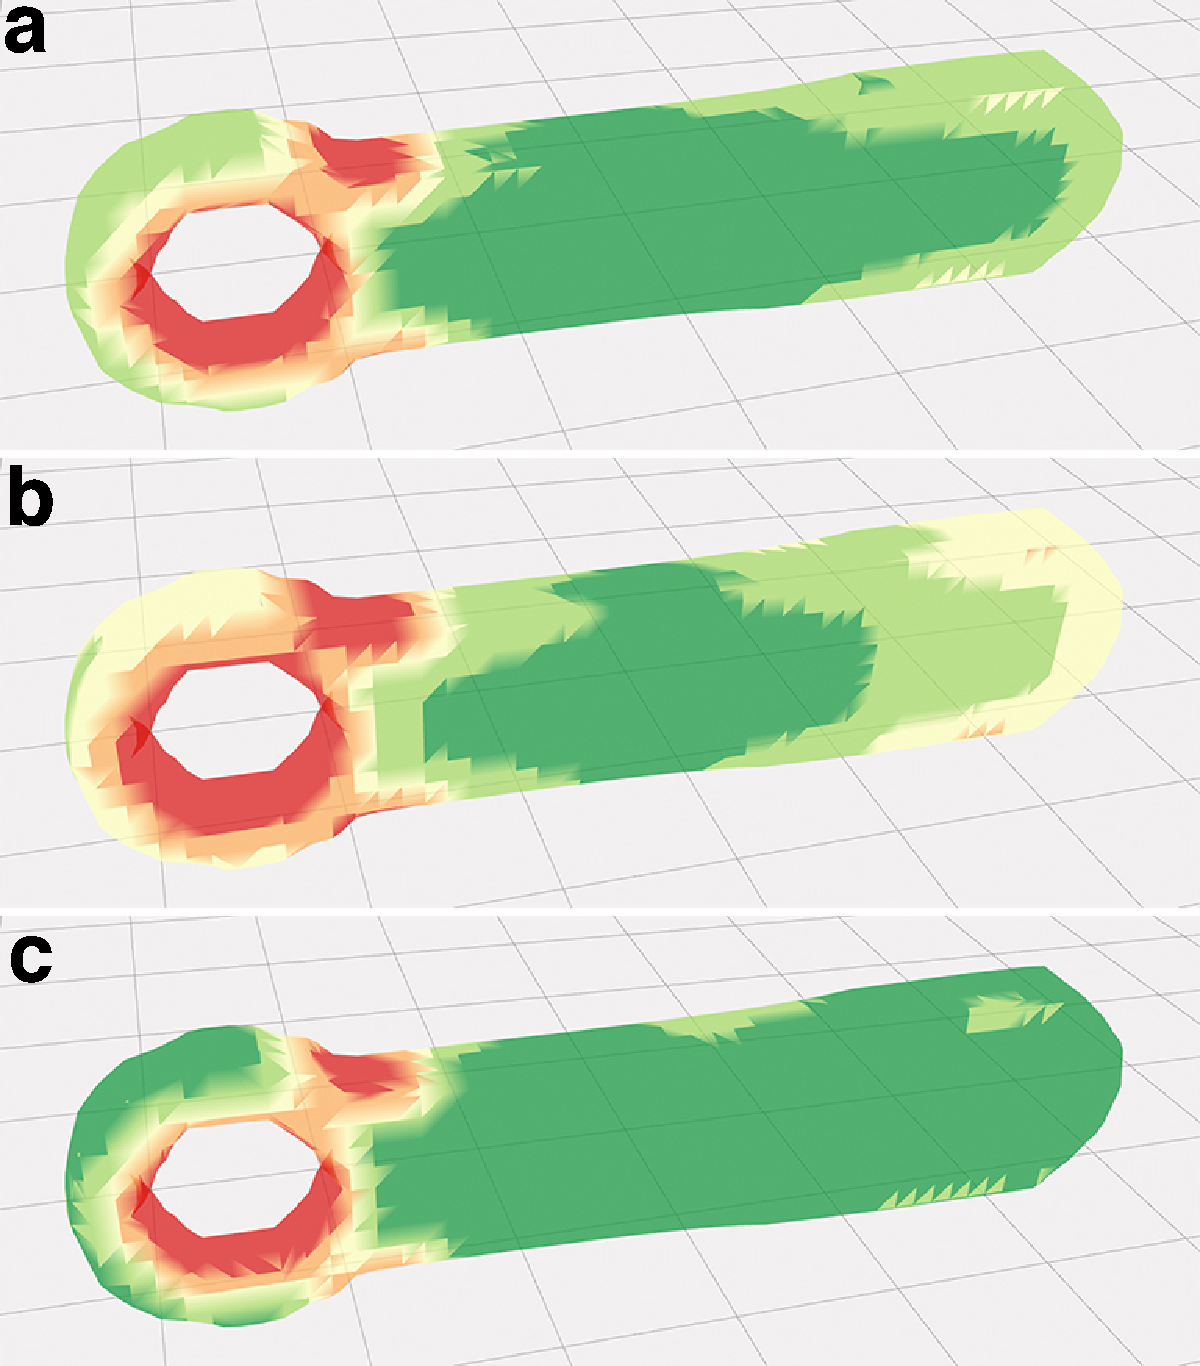
\includegraphics[width=0.6\textwidth]{figures/encore_visualization.pdf}
  \caption{A heat map is an effective way to visualize the analysis results for adding a handle to a wrench: a) red areas indicate a handle cannot be printed over (viability); b) emphasizing durability shows preference for areas with small curvature; and c) emphasizing balance (usability) shows preference for areas near the center of mass (This assumes the forces applied have the same direction as the surface normals).}~\label{fig:encore_visualization}
\end{figure*}

\subsubsection{Visualization Techniques}
Visualization provides effective feedback to the users to inform them about properties of their own design. When making attachments, one type of visualization is to compute an attachment score for each point on an existing object and overlay the results as we render the 3D model. Specifically, for each face on the object's mesh, we locate its neighborhood area $S$, and pre-compute the viability, durability and usability analysis for this area. The results from different analyses can be weighted and combined based on user input and the purpose of the attachment.

Figure~\ref{fig:encore_visualization} shows Encore's heat map visualization of these computed values, rendered on a wrench where the user would like to use print-over to add a handle (e.g., for hanging the wrench from a machine that needs frequent maintenance). The red areas indicate the parts of on the wrench where a handle cannot be printed over due to unavoidable occlusion (Figure~\ref{fig:encore_visualization}a). The user can adjust the weights given to the metrics, such as choosing to emphasize durability. The visualization is interactively updated and shows preference (green) for areas with small curvature (Figure~\ref{fig:encore_visualization}b). Alternatively, the user can emphasize balance, which narrows down the preferred areas to those near the center of mass (Figure~\ref{fig:encore_visualization}c).

\subsubsection{Direct Manipulation Techniques}
Some attachment techniques, such as strapping, might require more user direction. For example, Figure~\ref{fig:encore_feedback} shows in the print-through technique, how the user can position the existing object to interlock with the attachment. When the two meshes intersect with one another, the intersecting area is highlighted, which prompts the user to reposition the object to an intersection free location.
Another useful technique is to allow the user to draw on the existing object to specify the attachment area. For example, for affixing using straps, the user simply draws a stroke around part of the object to indicate a strap. Based on this partial strap, we can find the corresponding cross section by first finding a plane that best fits the stroke points, and then intersecting the object with the plane. Figure~\ref{fig:encore_interaction} shows an example of drawing to specify where to strap an attachment on a bottle.

\begin{figure*}[h]
  \centering
  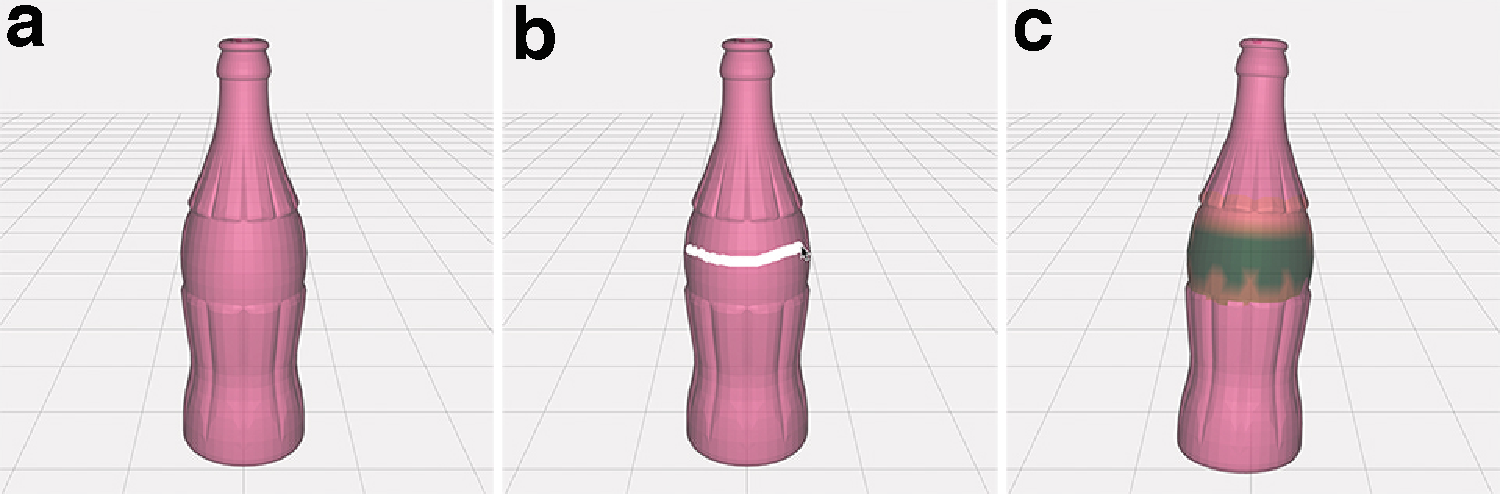
\includegraphics[width=0.8\textwidth]{figures/encore_interaction.pdf}
  \caption{Directly drawing on the object is a simple way to specify the attachment area, such as drawing a stroke around a bottle (a, b) to indicate where to attachment a strap. (c) a heat map visualization around the selected cross section. }~\label{fig:encore_interaction}
\end{figure*}

\subsection{Model Generation, Printing and Post-processing}
Once the user is satisfied with the attachment location, the pipeline continues to the last two phases: model generation, and printing and post-processing.

\subsubsection{Model Generation}
Model generation outputs a single file that includes the attachment, connector(s) and support structure. In particular, as discussed earlier, the connectors can raise the starting layer for printing the attachment to avoid potential occlusion issues; or be designed to snug-fit the existing objects (thus enabling affixing using adhesives or straps).

For some techniques, adding support can also solve occlusion problems. For example, in the print-through technique, when the attachment is much smaller than the existing object, it needs to be raised by a support structure so that the object can go through it while staying below the extruder. Other techniques use support to hold an object in place, such as direct print-over.

Figure~\ref{fig:encore_support}a shows a connector and the support structure for printing over a magnet holder on a Teddy bear (the same one shown in Figure~\ref{fig:encore_techniques}a). In this case, the five support cylinders at the bottom hold the bear in place and at the right orientation and have been prepared to exactly conform to the surface of the bear.

\begin{figure*}[h]
  \centering
  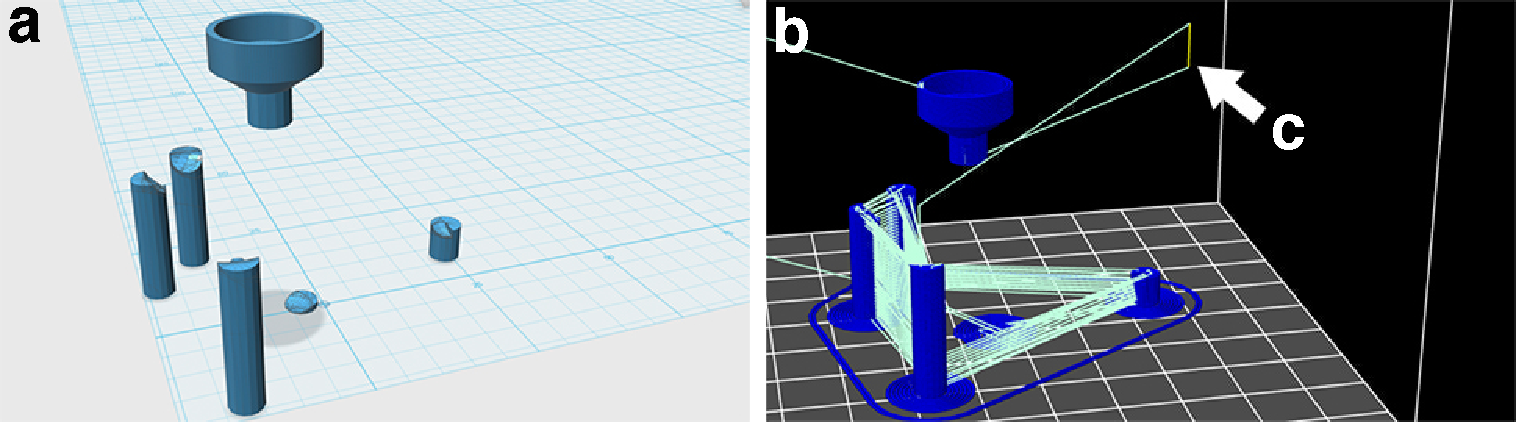
\includegraphics[width=0.9\textwidth]{figures/encore_support.pdf}
  \caption{In the Teddy bear magnet example, a) a model is generated with a magnet holder, a connector, and the support structure; b) Tool path view in Repetier-Host: the extruder pauses and moves away for inserting the teddy bear (c).}~\label{fig:encore_support}
\end{figure*}

\subsubsection{Printing and Post-Processing}
In the last phase, the user imports the generated models into the 3D printing tool chain for fabrication. Some attachment techniques require a simple customization of the printing process, which can be programmatically achieved using 3D printing software such as Repetier-Host\footnote{\url{http://www.repetier.com/
 }} (Figure~\ref{fig:encore_support}b). For example, both print-over and print-through require pausing the printer, inserting the existing object, and then resuming the print job. Having computed the pause point in the analysis, we can generate commands to perform these operations, such as:

\begin{verbatim}

G1 X0 Y0	; move the extruder away
G1 Z40		; raise the extruder
@pause		; pause the print for insertion
; print is manually resumed here after insertion
G1 Z31.550	; restore extruder's height

\end{verbatim}

Figure~\ref{fig:encore_support}c shows the extruder's tool path as a result of these few extra commands. The extruder makes room for the Teddy bear to be positioned onto the support structures. It then returns and finishes printing the magnet holder.

Finally, some techniques require a few post-processing steps after the attachment is fabricated, such as applying adhesives or straps to affix a new part that is printed separately from the existing object.

\subsection{Software and Hardware Implementation}
We have applied a computational framework--geometric analysis, interactive exploration, model generation, printing and post-processing supporting all three attachment techniques in Encore. Encore was implemented in JavaScript primarily using three.js\footnote{\url{http://threejs.org/}}--a library for programming with WebGL. All the attachment examples were fabricated by an FDM printer made from Printrbot's Simple Maker's Kit\footnote{\url{http://printrbot.com/shop/simple-makers-kit-2/}} . We used Slic3r\footnote{\url{http://slic3r.org/
 }} for G-code generation, Repetier-Host for communicating with the printer, and 1.75mm PLA as printing material in all our examples.

\section{Evaluation}
Below we report on an evaluation of our attachment approach from two perspectives: {\em (i)} to evaluate the printing process, we compare the cost of time and material for each technique; {\em (ii)} to evaluate the reliability of the printing results, we tested print-over and print-to-affix techniques, which rely on extrinsic adhesion ir fastening. Specifically, for these techniques, we investigate how well a fabricated handle can sustain forces that typically occur when holding, carrying and controlling an object.

\subsection{Evaluating Time and Material Cost}
One potential benefit of printing to augment existing objects rather than creating new ones is to spend less time and material printing. To verify this, we compare the printing plus processing time and material cost between our attachment techniques (print-over, print-to-affix, print-through) and a baseline approach, which prints a brand new object that has the attachment as an integral part of it.

\subsubsection{Cost Prediction Model}
As shown in Table 1 and Table 2, by the nature of different attachment techniques, we can predict how they differ in printing time and material cost.

Printing time is broken down to time spent on actual 3D printing (T) and time on handling or post-processing (t). For example, print-over requires the printing of the attachment, connector(s), and support structure; it also takes time to insert the existing object to be printed over, as well as to apply adhesives to increase the firmness of the scaffolding.

Material cost is split between printing the attachment and other structures. For example, print-through might also require support structures to keep the interlocking object collision free, even if the attachment itself does not have overhang problems.
For the baseline technique, printing time and material is spent on a new object made of the original object combined with the added attachment.

\begin{table}[h!]
\small
\centering
\caption{Prediction models for printing time of attachment techniques and data from a exemplar object+attachment. }
\label{tbl:encore_predtime}
\begin{tabular}{| c | c | C{9cm} | c |}
\hline
\multicolumn{2}{|c|}{\textbf{Technique}}   & \textbf{Prediction model for time}                                                & \textbf{\begin{tabular}[c]{@{}c@{}}Case study: \\ Utah teapot\end{tabular}} \\ \hline
\multicolumn{2}{|c|}{Print-over}           & $T_{attachment} + T_{connector} + T_{support} + t_{insert} + t_{apply\_adhesive}$ & 31:41                                                                       \\ \hline
Print-to-Affix & Adhesive & $T_{attachment} + t_{apply\_adhesive}$                                            & 13:56                                                                       \\ \cline{2-4}
                                & Strap    & $T_{attachment} + t_{strap}$                                                      & 11:27                                                                       \\ \hline
\multicolumn{2}{|c|}{Print-through}        & $T_{attachment} + t_{insert}$                                                     & 19:43                                                                       \\ \hline
\multicolumn{2}{|c|}{Print as one piece}   & $T_{attachment+object}$                                                           & 1:13:13                                                                     \\ \hline
\end{tabular}
\end{table}

\begin{table}[h!]
\small
\centering
\caption{Prediction models for material cost of attachment techniques and data from a exemplar object+attachment.}
\label{tbl:encore_predmat}
\begin{tabular}{| c | c | C{9cm} | c |}
\hline
\multicolumn{2}{|c|}{\textbf{Technique}}   & \textbf{Prediction model for time}                                                & \textbf{\begin{tabular}[c]{@{}c@{}}Case study: \\ Utah teapot\end{tabular}} \\ \hline
\multicolumn{2}{|c|}{Print-over}           & $M_{attachment} + M_{connector} + M_{support}$ & 916mm                                                                      \\ \hline
Print-to-Affix & Adhesive & $M_{attachment}$                                            & 402mm                                                                       \\ \cline{2-4}
                                & Strap    & $M_{attachment}$                                                      & 396mm                                                                     \\ \hline
\multicolumn{2}{|c|}{Print-through}        & $M_{attachment} + M_{support}$                                                     & 582mm                                                                      \\ \hline
\multicolumn{2}{|c|}{Print as one piece}   & $M_{attachment+object}$                                                           & 3054mm \\ \hline
\end{tabular}
\end{table}

\subsubsection{A Case Study}
We verify these intuitions in a concrete attachment case: adding a torus-shaped handle to the Utah teapot. We chose the Utah teapot because it is a classic 3D model and because it is also one of the few widely used 3D models where all of our techniques are applicable. The results are shown in Table~\ref{tbl:encore_predtime} and Table~\ref{tbl:encore_predmat}.

The goal of this evaluation is to reveal how time and cost differ between various techniques, rather than to obtain a `true' value through repetitive trials. As such, we used the slicer program (Slic3r) to estimate printing time and material cost. This program calculates time and cost as it analyzes the input models and generates the corresponding G-code. For techniques that require handling or post-processing, such as applying adhesive, we empirically estimate the time. The particular adhesive we chose (Loctite “Professional Heavy Duty” Epoxy Loctite \#1172794 requires 5 minutes of `setting' time, while strapping usually takes no longer than 3 minutes.

Both the prediction model and case study results support our intuition--when support is needed, time and materials go up; and the baseline condition is dominated by the time needed to print the existing object.

To better understand the tradeoffs, we conducted another evaluation to test the general strength of our print-over and print-to-affix, also compared to the same baseline (an integral print of existing object and attachment). Print-through is often done loosely without binding between surfaces. Thus strength issues for print-through are directly related to the objects themselves, rather than the attachment technique. Similarly, print-to-affix using adhesives depends heavily on properties of the adhesive used. As such, no testing was performed for these two techniques. We report on print-over and print-to-affix using strapping.

\subsection{Evaluating the Strength of Printed Attachments}
The goal of this evaluation is to understand the tradeoffs and limits of our techniques in comparison to each other. We tested a type of attachment – handles, as they are likely to experience external forces, such as holding, gripping or pulling. For each attachment technique tested, we fabricated handles using the same printer and material as described earlier. Similar to \cite{umetani2013cross}'s test of printed objects' cross sectional strength, we exerted a bending force tangential to each handle's attachment point (pulling the handle sideways at $90^{\circ}$ with respect to its main axis, as illustrated in Figure~\ref{fig:encore_eval_scene}). We then gradually increased the force and measured the point of fracture \cite{tetelman1967fracture}.

\subsubsection{Evaluating Print-Over Attachment}
For testing print-over attachment, we designed a torus-shaped handle with fixed outer radius of 7.5 mm and inner radius of 2.0 mm. We empirically set these values to match the size of human fingers. Larger scales of handles are much more time-consuming to fabricate and might go beyond the dimension limit of our printer. Thus we leave them for future work.

We then computationally generated a series of 20mm by 20mm by 5mm platforms whereon to fabricate the torus handles, connected via a cylindrical connector (radii: 1.5mm, height: 3mm).

Next we modified the top surfaces of these platforms: the independent variables are the Curvature and Roughness of these top surfaces.

\begin{figure*}[h]
  \centering
  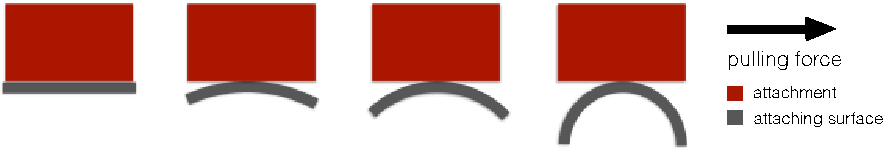
\includegraphics[width=0.9\textwidth]{figures/encore_eval_printover.pdf}
  \caption{To test print-over in comparison to printing in one piece, we used both techniques to print attachments on surfaces with varied curvatures and then exerting tangential pulling force.}~\label{fig:encore_eval_strap}
\end{figure*}

\begin{itemize}
\item Curvature. Assume $R$ is the radius of a platform's top spherical surface and $r$ is the radius of the cylindrical connector of the handle. We modeled the curvature by $C = r/R$. Specifically, we tested on $C$ = 0 (a flat surface), 0.25, 0.5, and 1.

\item Roughness. We performed Boolean subtraction operation between the platform's top surface and a pre-set number $N$ of small spheres whose centroids are on the surface, positions randomized, and radii randomly distributed in [0.25mm, 1mm]. This made the surface porous, thus creating roughness. We tested on $N$ = 0 (smooth surface), and 10 (rough surface).
\end{itemize}

We fabricated the platforms and handles under these conditions using print-over and the baseline print-in-one-piece approach.

As shown in Figure~\ref{fig:encore_eval_scene}, we clamped the platform firmly onto the top of a table so that the handle was pointing upward. We then used a handheld scale to hook and pull the handle horizontally. We used a slow uniform motion for increasing the force. The process was videotaped to capture the scale's reading at the moment when the handle fractured or detached. We performed three trials for each condition.

\begin{figure*}[h]
  \centering
  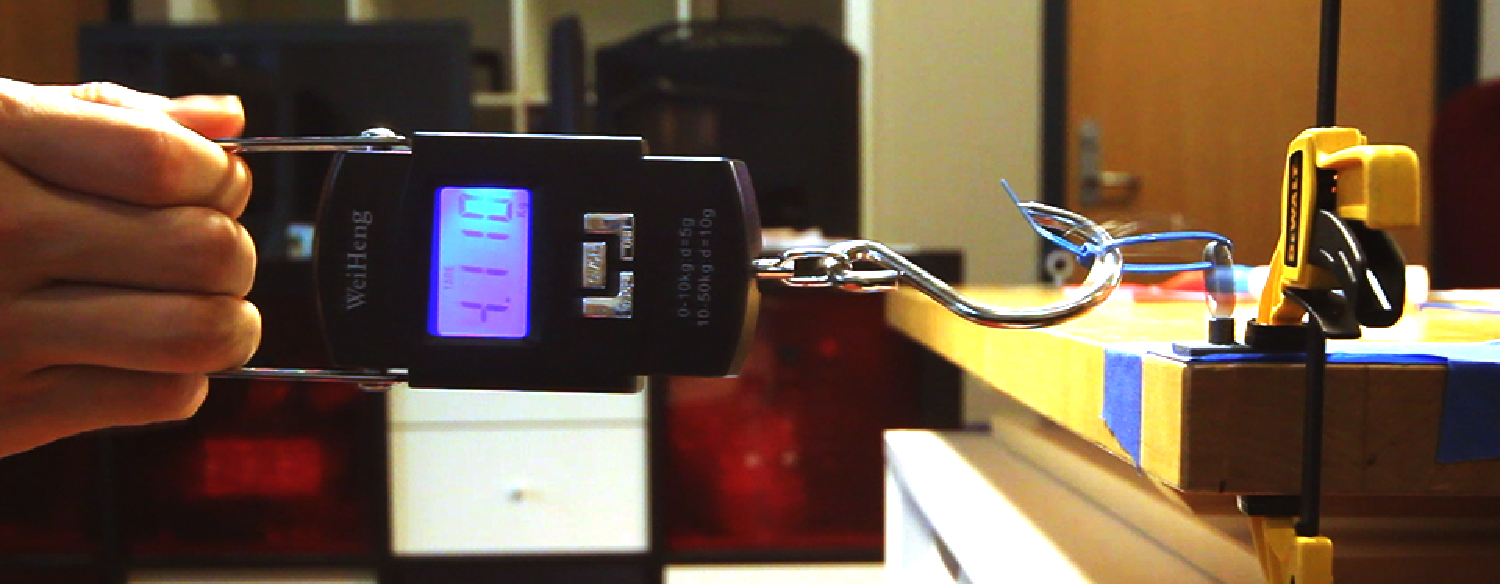
\includegraphics[width=0.9\textwidth]{figures/encore_evaluation_scene.pdf}
  \caption{Testing the strength of a 3D printed handle attachment (b) by clamping it on a table (c) and pulling using a scale to measure force (a).}~\label{fig:encore_eval_scene}
\end{figure*}

Figure~\ref{fig:encore_eval_result} shows the results of the strength test: overall print-over's best performance was close to that of the baseline. However, it suffered from an increase of surface curvature (Figure~\ref{fig:encore_eval_result}a) and roughness (Figure~\ref{fig:encore_eval_result}b).

\begin{figure*}[h]
  \centering
  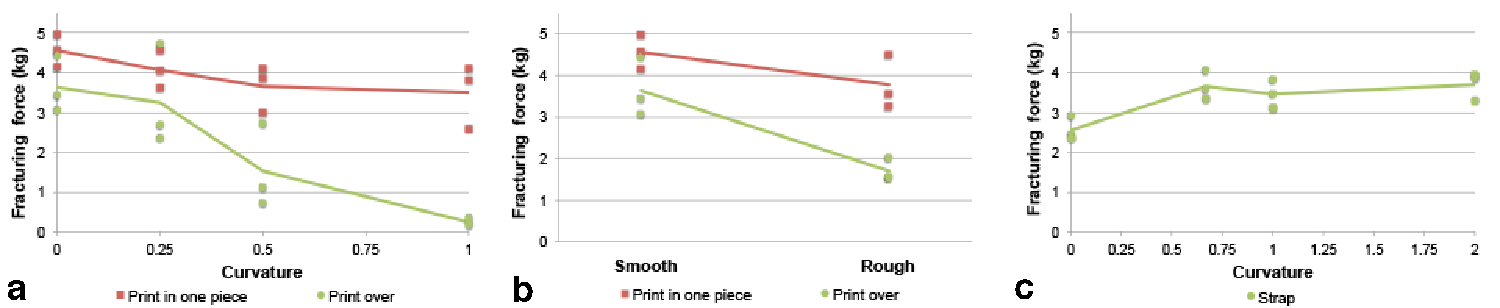
\includegraphics[width=1\textwidth]{figures/encore_evaluation_results.pdf}
  \caption{Strength test results show print-over is strong enough to sustain stress as if they had been printed in one piece. Both our techniques suffer from an increase of surface curvature (a) and roughness (b); (c) shows that affixing with straps (150mm zip tie) is able to sustain over 2.5 kg of pulling, and reacts differently to curvature. }~\label{fig:encore_eval_result}
\end{figure*}


Affixing using adhesion is also related to this evaluation. However, its performance is hard to test in a general way, as it strongly depends on the particular types of adhesives used, as well as the user's experience and expertise of handling it. Therefore we leave it as future work.

\subsubsection{Evaluating Strapping-based Attachment Techniques}
Using straps requires a different analysis than print-over. The key question for strapping is how likely the object is to ‘slip' through the strap when pulling forces are exerted. This is a potential issue that does not occur with the baseline and adhesive attachment mechanisms. Thus we tested this affixing technique independently of the other attachment options.

Specifically, given the same cross section $S$ (we use a circular $S$), we are interested in whether and how the curvature perpendicular to $S$ affects `strappability'. To test this, we computationally generated a series of olive-shaped objects created by revolving a circular segment (with radius $R$) around its secant. We computed the secant so that the revolved shape had a cross section of radius L/2. We then symmetrically cut off the two ends of so that the remaining pieces have a uniform length of $L$.

We quantified curvature as $C = L/R$. We tested $C$ = 0 (a cylindrical lateral area), 0.67, 1, and 2. For each object, we generated a handle attachment using Encore, and then fabricated it and strapped it around the center of the object using a 150mm zip tie. We then firmly clamped the handle to a table and then pulled on the strapped object, measuring the minimal force required to pull the test object out of the strap using a similar setup as the previous test (Figure~\ref{fig:encore_eval_strap}).

\begin{figure*}[h]
  \centering
  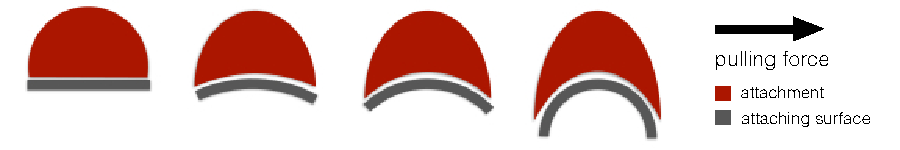
\includegraphics[width=0.9\textwidth]{figures/encore_eval_strap.pdf}
  \caption{To test strapping in print-to-affix, we increased the curvature between the attachment and the attaching surface and exerted tangential pulling force.}~\label{fig:encore_eval_strap}
\end{figure*}

Figure~\ref{fig:encore_eval_result}c shows the test results. Depending on the curvature, a 150mm zip tie attached using our approach can sustain a pulling force of from 2.5 to 4 kg without letting the object slip. Interestingly, strapping strength improved with increased curvature (Figure~\ref{fig:encore_eval_result}c), in contrast to other attachment methods (Figure~\ref{fig:encore_eval_result}a).

\section{Summary of Attachment Techniques}
Although the tested attachment techniques were developed using the same framework, our performance testing demonstrates that they have their own unique advantages and weaknesses. A limitation of our evaluation is its focus on 3D printed existing objects. In this discussion we provide some anecdotal intuition about other factors that might affect the reliability of attachments fabricated by our techniques. Further, to better understand these techniques as a whole, we also discuss some practical issues in comparison with one another.

Print-over, as shown in our evaluation, creates strong adhesion between attachments and objects that are made of the same or very similar material. It also requires no post-processing. However, it has weak adhesion on some materials. For example, when making the LED torch (Figure~\ref{fig:encore_overview}a), our initial attempt to directly print on the metal shell of the battery was not successful. The problem was eventually solved by the simple addition of a thin layer of glue on top of the battery shell. We expect that the use of a glue layer will show promise in other situations as well, but substantially more experimentation and testing is required before its range and properties can be precisely understood.

Affixing with adhesives is widely applicable to a range of geometry and material. But it requires good selection of adhesives, and in some cases careful handling of the amount and mixing of ingredients in order to achieve the best adhesion. Compared with the other techniques (e.g., print-over and print-through), affixing with adhesives relies perhaps the most on the expertise of the users.

Affixing with straps is easily adjustable and also makes an attachment reusable. However, it could be less aesthetically desirable for some use cases. Surprisingly, within the range of our tests, as curvature increased strapping attachment became stronger, whereas all other techniques became weaker. We hypothesize that when the interface between the existing object and the compliant strap has higher curvature, it requires more deformation of the strap in order for the object to slip. Thus the strap can sustain a higher pull force when the curvature increases. However, this hypothesis requires more investigation.

Print-through is a natural attachment mechanism that requires no adhesion or fastening. However, it has limited scope of use as only some objects have appropriate holes or loops that are required to perform this technique.

Despite its increasing popularity, 3D printing has been used almost exclusively to create objects `from scratch', rather than leveraging things that already exist in our day-to-day life. In this project, we present a framework for using 3D printing to augment everyday objects, and provide specific analytical and computational support for realizing one approach of augmentation – adding functional attachments to existing objects. Our framework encompasses key aspects of attachment including geometric analysis, interactive exploration, model generation, and printing and post-processing support. In particular, we present an extensible set of analytical techniques, all based on the geometric form of the existing object and the proposed attachment, and range from very general print viability issues, to durability issues, to very specific usability issues.

There are several remaining questions that require further investigation. Foremost, are there any other attachment techniques that can leverage the use of a 3D printer? Are there any new perspectives that could be introduced into the analyses? Are there any specific use of adding attachments to existing objects that might require further computational support? In my next project, I focus on exploring the third question: I go from developing attachment techniques to enabling the design of functional attachments that can adapt real world objects for custom use.

Another question is given these attachment techniques, how we can design add-on components so that they can serve to augment an object in user-customized ways. My next chapter answers this question through the exploration of designing 3D printed adaptations---components that mechanically enhance or repurpose an existing object.
